%%--------------------------------------------------------------------------
%% INTRODUCTION
%%--------------------------------------------------------------------------



\subsection{Introduzione}


\subsubsection{Scopo del documento}
Lo scopo di questo documento è quello di mostrare le scelte implementative fatte durante lo sviluppo dell'applicazione \textit{Incastri Sonori 2}. Esso si divide in $3$ sezioni: \textit{Database}, \textit{Logica di gioco}, e \textit{Interfaccia Utente}.

\subsubsection{Descrizione dell'applicazione}
\textit{Incastri Sonori 2} è un videogioco per piattaforma Android progettato esclusivamente per dispositivi tablet. Lo scopo del gioco è quello di comporre parole a partire da tessere colorate rappresentanti diverse sillabe. Ogni tessera ha un colore associato direttamente alla sillaba che rappresenta e non appena viene toccata il dispositivo riproduce (tramite il sintetizzatore vocale) il suono della sillaba. Toccando due tessere una dopo l'altra è possibile comporre una parola che, se corretta, verrà aggiunta all'elenco delle parole trovate sotto forma di immagine composta dalle due tessere. La schermata consente inoltre di riascoltare le parole trovate, sia in italiano sia in inglese. Una partita può essere composta da più schermata; ogni schermata termina quando sono state trovate tutte le parole componibili con le sillabe mostrate (2 o 4).\\
Durante il corso della partita l'applicazione registra i tempi in cui vengono identificate le parole, e le invia ad una mail configurabile nelle impostazioni.\\
E' presente inoltre una modalità cooperativa a due giocatori a turni. Ogni turno consente ad un giocatore un tentativo per indovinare una parola.\\
La figura \ref{fig:play_ui} mostra l'interfaccia di gioco.

\begin{figure}[h!]
\label{fig:play_ui}
  \centering
    \centering{
      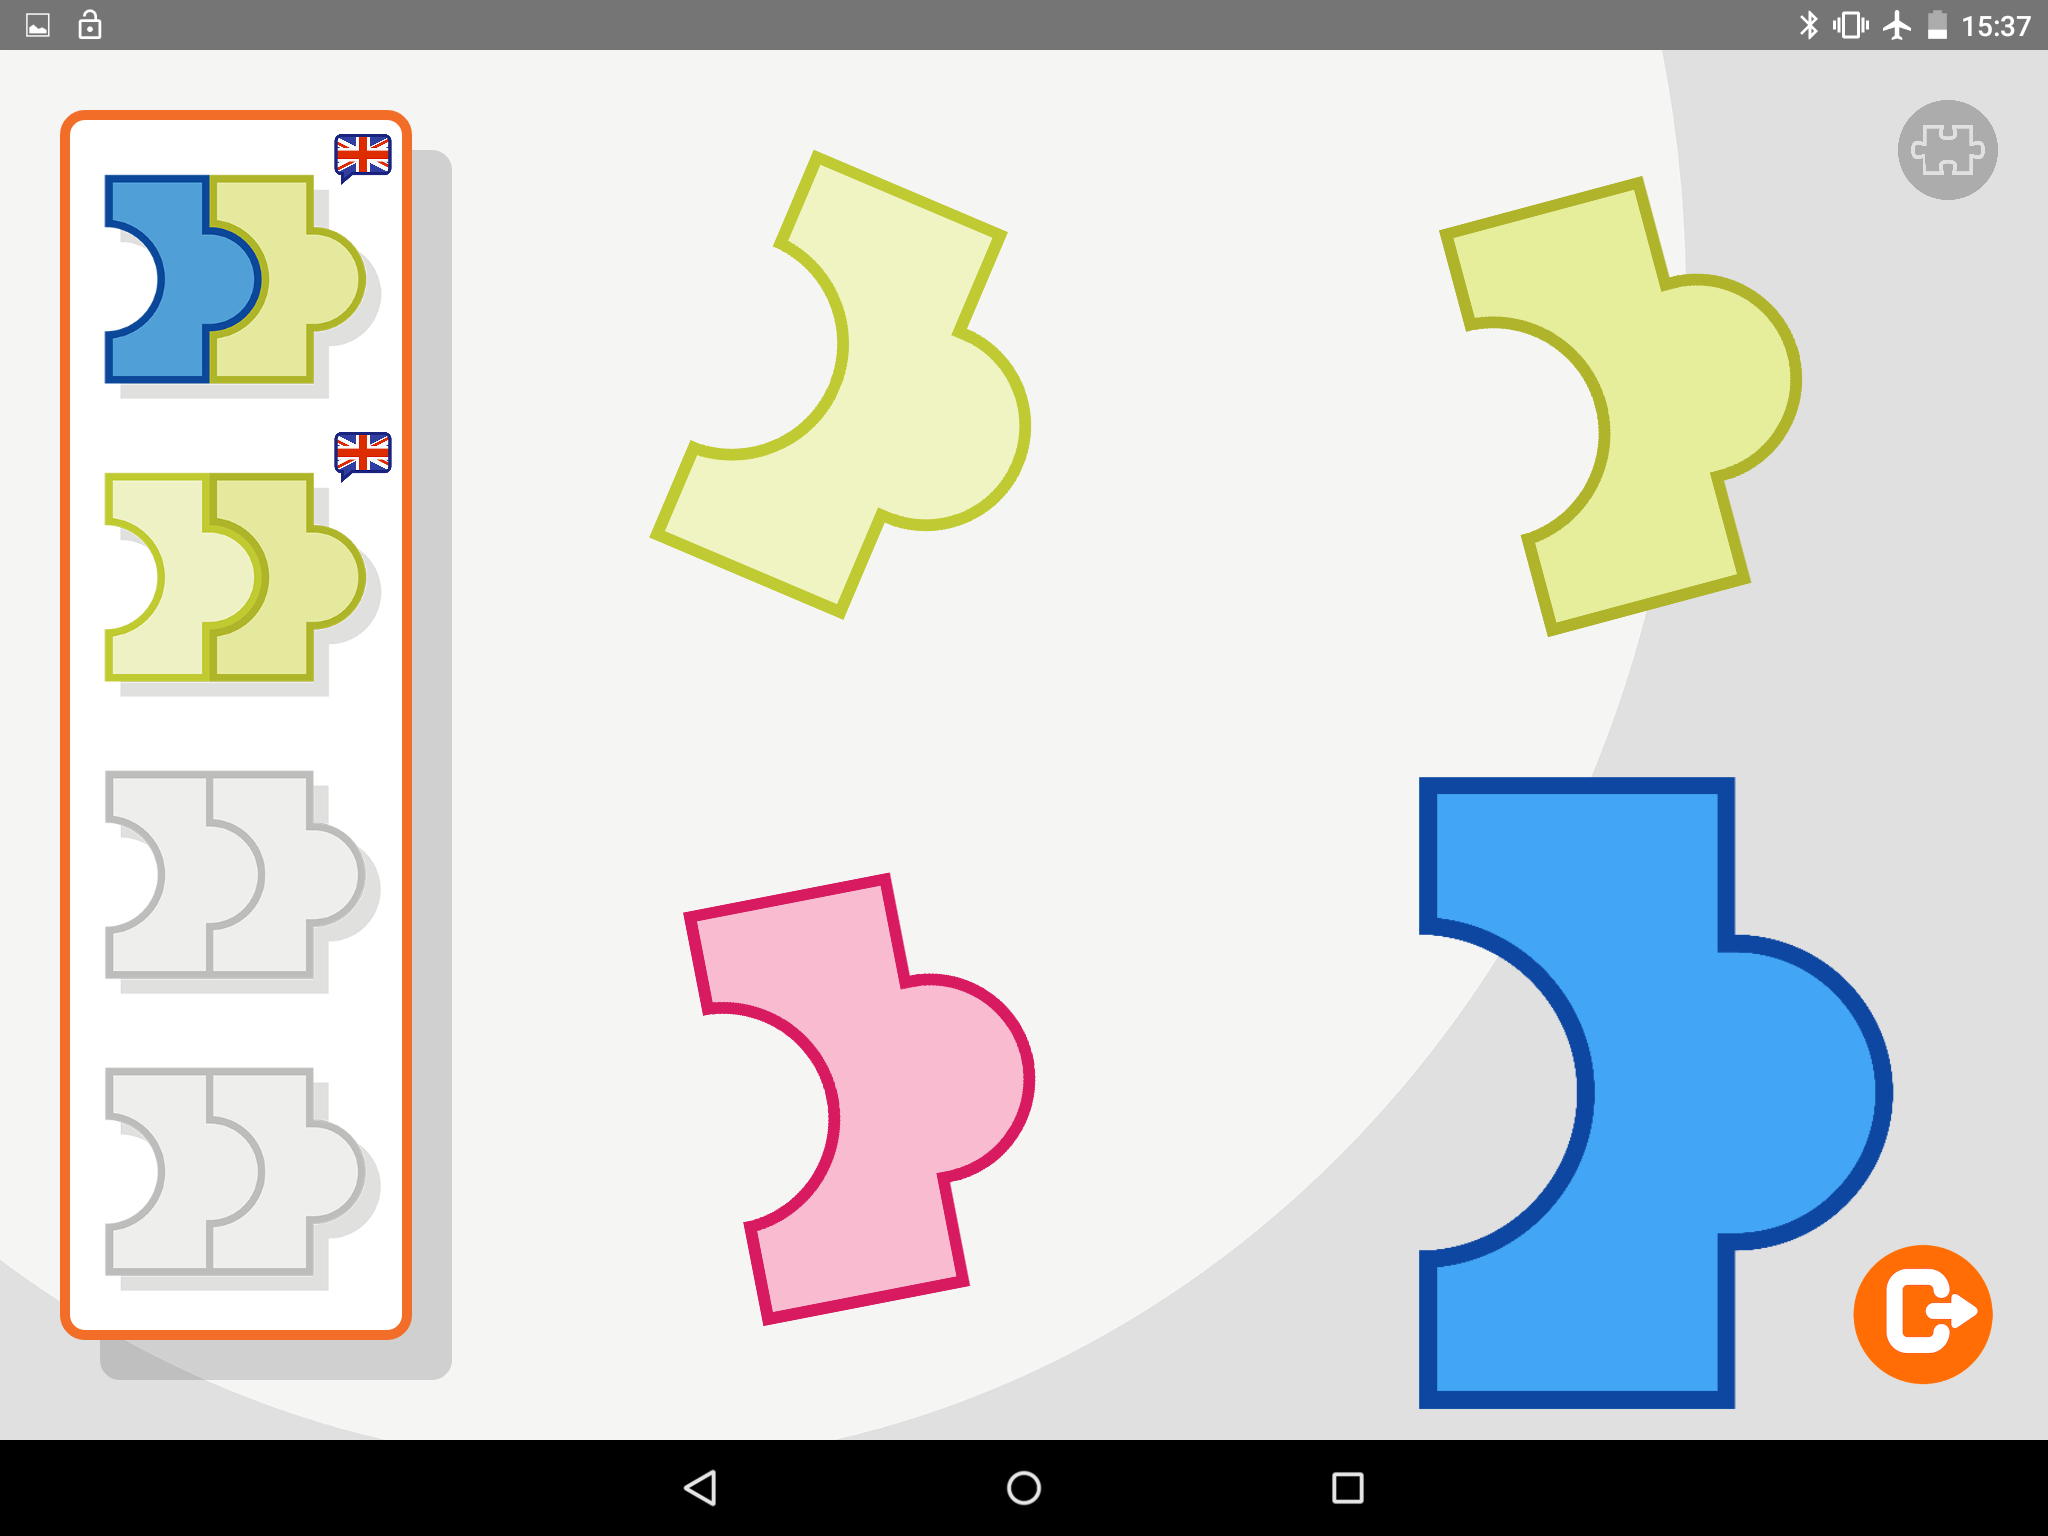
\includegraphics[width=\textwidth]{play_ui.png}}
  \caption{Schermata di gioco}
\end{figure}
